\documentclass[review,authoryear]{elsarticle}

\usepackage{lineno,hyperref,amsmath,amssymb,graphicx,tikz}
\usepackage{comment}
\usetikzlibrary{fit}
\newcommand\addvmargin[1]{
  \node[fit=(current bounding box),inner ysep=#1,inner xsep=0]{};
}
\modulolinenumbers[1]

\journal{Journal of Theoretical Biology}

%%%%%%%%%%%%%%%%%%%%%%%
%% Elsevier bibliography styles
%%%%%%%%%%%%%%%%%%%%%%%
%% To change the style, put a % in front of the second line of the current style and
%% remove the % from the second line of the style you would like to use.
%%%%%%%%%%%%%%%%%%%%%%%

%% Numbered
%\bibliographystyle{model1-num-names}

%% Numbered without titles
%\bibliographystyle{model1a-num-names}

%% Harvard
%\bibliographystyle{model2-names.bst}\biboptions{authoryear}

%% Vancouver numbered
%\usepackage{numcompress}\bibliographystyle{model3-num-names}

%% Vancouver name/year
%\usepackage{numcompress}\bibliographystyle{model4-names}\biboptions{authoryear}

%% APA style
%\bibliographystyle{model5-names}\biboptions{authoryear}

%% AMA style
%\usepackage{numcompress}\bibliographystyle{model6-num-names}

%% `Elsevier LaTeX' style
\bibliographystyle{elsarticle-harv}
%%%%%%%%%%%%%%%%%%%%%%%
\makeatletter
\newcommand*{\rom}[1]{\expandafter\@slowromancap\romannumeral #1@}
\makeatother
\begin{document}

\begin{frontmatter}

\title{Analysis of tumor-immune functional responses in a mathematical model
of cancer vaccines}


%% Group authors per affiliation:
\author{Elsevier\fnref{myfootnote}}
\address{Radarweg 29, Amsterdam}
\fntext[myfootnote]{Since 1880.}

%% or include affiliations in footnotes:
\author[mymainaddress,mysecondaryaddress]{Elsevier Inc}
\ead[url]{www.elsevier.com}

\author[mysecondaryaddress]{Global Customer Service\corref{mycorrespondingauthor}}
\cortext[mycorrespondingauthor]{Corresponding author}
\ead{support@elsevier.com}

\address[mymainaddress]{1600 John F Kennedy Boulevard, Philadelphia}
\address[mysecondaryaddress]{360 Park Avenue South, New York}

\begin{abstract}
Cancer neoantigen vaccines have emerged as a promising way to stimulate
the immune system to fight cancer. We present a phase plane analysis
of a simple model to understand immunological mechanisms of
cancer neoantigen vaccines. Analytical results are obtained for
two widely used killing terms of tumor cells by immune cells:
the law of mass action and the dePillis-Radunskaya Law. For the law
of mass action killing, we derive a result that offers an alternative
explanation of sneaking through of a slowly growing tumor. Moreover,
the existence of a unique periodic solution is shown. The dePillis-Radunskaya
Law offers richer dynamics, for which tumor elimination and uncontrolled growth are both present. We show that the elimination of a tumor depends
on initial conditions, which provides support for using cancer vaccine
as an adjuvant therapy after the primary tumor is reduced by surgery
or radiotherapy. A sufficient condition for uncontrolled tumor growth 
is also derived for the dePillis-Radunskaya Law. 
\end{abstract}

\begin{keyword}
cancer vaccines \sep XX \sep XX
%\MSC[2010] 00-01\sep  99-00
\end{keyword}

\end{frontmatter}

\linenumbers

\section{Introduction}

The immune system plays an important role in controlling tumor growth
and progression to malignancy \citep{Waldman2020}. Innate and adaptive
immune responses are two types of immune response. The immune system
launches these responses to fight against cancer. As a tumor acquires
cancerous mutation, it starts expression of non-synonymous mutations
that produces tumor-specific antigens called neoantigen \citep{Peng2019}.
Neoantigen can be recognized by the immune system and induces adaptive
immune responses (elaborate?). This includes proliferation of T cells
that specifically kill the tumor cells associated with the particular antigen.
However, the immune response naturally induced may not be present
or sufficient in cancer patients to control tumor growth. Immunotherapy
is a type of cancer treatments that assists the immune system in fighting
against cancer. With the advance in genome sequencing, neoantigen
cancer vaccine, that is designed to target specifically tumor cells
by recognizing their neoantigen, has emerged as a promising way to
treat cancers. This modality, which works by injecting synthetic tumor-specific
peptides into the patient to activate peptide-specific T cells, is
highly personalized and has shown its strength in avoiding auto-immune
side effects \citep{Nelde2021} and achieving desirable clinical outcomes in
treating different cancers (such as FDA approved prostate cancer vaccines)
\citep[e.g.][]{Ott2017,Pan2018,Peng2019}. 

The complexity of the immune system and its interactions with tumors
makes it challenging to understand their dynamics and design optimal
immunotherapy treatments. Mathematical modeling is valuable in enhancing
our understanding of tumor-immune interactions. Numerous successes
of mathematical modeling can be found in the vast literature on this
subject \citep[e.g. see reviews by][and references therein]{Eftimie2016,Mahlbacher2019,Nukala2021}. Mathematical models can be used for hypothesis
generation because the mechanisms accounted for by the models. Their
quantitative nature also make them useful in making predictions and
optimizing treatments. 

On the topic of modeling immunotherapy or cancer immunology, ordinary
differential equations (ODEs) is arguably the most popular choice
given its simplicity and analytical or computational tractability
\citep{Eftimie2010}. The size of ODE models ranges from one or few
equations to more than a dozen equations. Even in developing a large
ODE system, it is inevitable that the modeler has to focus on certain
aspects of cancer immunology or immunotherapy. One of the most important
aspects is the interaction between the tumor and the immune system, especially
how tumor cells are reduced by the immune system. For example, predictor-prey
systems are often used to model this interaction where tumor cells
are prey and effective immune cells are predators \citep{Hamilton2022}. The growth of tumor is well studied in mathematical
models, which takes form such as exponential, logistic and Gompertizian
growth \citep{Murphy2016}. In contrast, the killing of tumor cells
by immune cells are less often studied. It is frequently modeled using
the law of mass action, popularized by the seminal paper by \citet{KUZNETSOV1994}.
Another common choice of the killing term is the so-called dePillis-Radunskaya
Law proposed by \citet{dePillis2014} who showed it fits some data
better (word choice?). The law of mass action based on the well-mixed
assumption stems from chemical reactions. To our knowledge, the dePillis-Radunskaya
Law is purely phenomenological. In fact, there is no governing laws
of biology {[}{]}. Both choices have some merits and shine in different
circumstances. The dePillis-Radunskaya Law is more likely to be a
better choice than that based on the law of mass action when well-mixed
assumption is less reasonable. Oftentimes, the data is not enough
to draw a conclusion about which to choose. The selection usually depends on the preference
of the modeler and is not often sufficiently justified. The difference in dynamics
as a result of choosing one functional form over the other is not
clear. 

In dealing with increasing complexity of mathematical models and growing
needs to use them to inform decision-making for public health, \citet{Basu2013} urged that sensitivity analysis should
not only be done with parameters but also on the alternative structures
of the model. Particularly, we recognize enormous efforts devoted
in modeling cancer immunotherapy with the goal to inform medical treatments
while there is a lack of attention on modeling choice of some key
model components. Cancer vaccine is inherently a personalized
therapy. Personalization is often reflected in modeling as patient-specific
parameters. Yet it is reasonable to expect parts of the cancer heterogeneity
may be better accounted by differences in model structures (remove?).
This has potential to explain the various levels of success of cancer
vaccine in different patients and for different types of cancers. We
hope that this paper will bring more awareness of potential opportunities
and issues on this front. We believe that more mechanistic justification
is needed for model selection although the killing of tumor by immune
system is often modeled phenomenologically.

The objective of this paper is to investigate analytically the consequence
and implications offered by two choices of killing terms in a simple mathematical
model of cancer vaccines. Specifically, we are interested in learning
how the functional form of the killing term may lead to tumor elimination
or uncontrolled growth (i.e., tumor escapes the immune control). We present
a model of a system of three ODEs
including three species: vaccine peptides, activated T cells, tumor
cells, as a simple alternative to the model proposed by \citet{Messan2021}. By a quasi-steady state (QSS), the system is further reduced
to two equations. Our phase plane analysis and close-form analytical
results offer clear biological interpretations, which complement the
the simulation-based study by \citet{Messan2021}. 

The paper is organized as follows. In section \ref{sec:A-simplified-model},
we introduce a simple mathematical model and make assumptions and approximations
needed to prepare the system for analysis. In section \ref{sec:data}, a rudimentary data fitting and exploratory analysis are conducted, which motivate further mathematical analysis of the model. In section \ref{sec:Analysis-on-two},
we perform analysis of the reduced model to contrast the resulting
difference in dynamics by the law of mass action verse the dePillis-Radunskaya
Law killings. In section \ref{sec:Discussion}, we discuss the biological
meaning implied by the two different killing terms, recognize the
limitation in the current work and point out future directions. 



\section{Model description \label{sec:A-simplified-model}}

We propose a simple model as an alternative to the model by \cite{Messan2021} as follows
\begin{subequations}\label{eq:3sp-model}
\begin{eqnarray} 
P' & = & D(A,T)T-\delta_{P}P+u(t)\label{eq:P'}\\
A' & = & a(P)-\delta A\label{eq:A'}\\
T' & = & \beta T-mD(A,T)T\label{eq:T'}
\end{eqnarray}
\end{subequations}
where prime($'$) indicates time derivative $\frac{d}{dt}$ (we will
use this shorthand notation for derivatives henceforth and the independent
variable with respect to which the derivatives is taken should be
clear in the context), $P, A$ and $T$ denote neoantigen peptides,
activated T cells and tumor cells respectively. In comparison to \cite{Messan2021},
the following simplification are assumed
\begin{itemize}
\item constant supply of naive cells is assumed \iffalse (to do: refs) \fi
\item CD4+ and CD8+ T cells are lumped into one species, the activated T
cells 
\item the detailed antigen presenting process by dendritic cells are left
out and proliferation of activated T cells are modeled phenomenologically
as a function of $P$.
\end{itemize}
The term $D(A,T)T$ appears in both (\ref{eq:P'}) and (\ref{eq:T'}).
In (\ref{eq:T'}), it represents the killing of tumor cells by the
activated T cells. As a result of lysis of tumor cells, neoantigen
peptides are released \citep{Konstorum2017} and hence it appears in
(\ref{eq:P'}) as a production term. It is reasonable to require that
$D(A,T)$ increases with $A$ and decreases with $T$. In this paper,
we will focus on two forms of $D$
\begin{itemize}
\item the law of mass action $D(A,T)=A$;
\item the dePillis-Radunskaya Law 
\begin{equation}
D(A,T)=\frac{(\frac{A}{T})^{n}}{k^{n}+(\frac{A}{T})^{n}}\label{eq:PR law-1}
\end{equation}
which has a range $(0,1)$. 
\end{itemize}
In absence of T cells, the growth of tumor cells is assumed to be exponential
with rate $\beta$ . This is no doubt a simplification. In reality,
tumor cells without interventions may undergo a stage of exponential
growth but exponential growth cannot be sustained because various
constraining factors such as space, oxygen or other immune controls not considered in this work.
In the modeling literature, logistic  \citep[e.g.][]{DePillis2013,Nikolopoulou2018}
and Gompertizian growth \citep[e.g.][]{Norton1988,Castillo2015} 
are popular choices as well as power law growth \citep{Dethlefsen1968}.
There are studies dedicated to comparing different approaches in modeling
tumor growth \citep{Murphy2016}. Despite the popularity of other
choices, it is frequent to find exponential growth being used to model
tumor growth, which has merit in its simplicity. In our formulation,
choosing exponential growth allows us to focus on the effects of different
choices of killing terms. The consequence of unbounded solution of
tumor population $T$ can clearly be interpreted as failure of the
treatment or death of the patient. 

In (\ref{eq:A'}), $a(P)$ models the conversion of the naive T cells
to the activated T cells when neoantigen peptides are present, which is
one of the types of immune activation (IA) and the only one considered
in this work. This is a simplification we take being aware of a well
known fact that neoantigen piptides need to be processed and presented
by antigen presenting dendritic cells to activate T cells. It is reasonable
to require that $a(P)$ increases with $P$. We start numerical experiments
in MATLAB R2021a using Hill functions for IA, i.e. 
\begin{equation} \label{eq:hill-a(P)}
a(P)=\phi P^{\lambda}/(s^{\lambda}+P^{\lambda}), 
\end{equation}
which is widely used to model activation in biology.

Naturally peptides decay as represented in our model with rate $\delta_{P}$.
We do not specify a multiplying parameter in front of $D(A,T)T$ in
(\ref{eq:P'}) because peptides $P$ are a latent variable in our data set and scaling
can be applied to remove the multiplying parameter without loss of
generality.



\section{Data fitting and exploratory analysis} \label{sec:data}
We first perform data fitting on the full model (\ref{eq:3sp-model}) with the law of mass action killing. Patient-specific parameters are estimated by minimizing residual sum of squares (RSS) on the same data set used by \cite{Messan2021}, which consists activated T cell counts of 6 patients treated with cancer vaccines. Here $\beta, \delta, s$ and $\phi$ are deemed to be patient-specific. Due to sparsity of data, especially that $P$ and $T$ are latent variables, it is not surprising to find other parameters unidentifiable.  Since the model lumps many intermediate biological processes and is phenomenological on its construction, it is unwise to attempt to look up the exact values for those parameters in the literature. We fix those parameters with our best guesses. In Fig. \ref{fig:data-fitting.}, we find the model fits the data reasonably well. Moreover, the model prediction shows patient 2 and 6 do not respond to the cancer vaccine well, which agrees with the observation that they both developed metastasis after the treatment. All parameters are reported in Table \ref{tab:parameters} as well as RSS in comparison to that of the model by \cite{Messan2021}. \cite{Messan2021} originally reported adjusted $R^2$. Due to the controversy of using $R^2$ as a metric for nonlinear models \citep{Spiess2010}, we convert their $R^2$ to RSS and find them  in par with ours (see last two rows of Table \ref{tab:parameters}). 

We find that the model with the dePillis-Radunskaya Law killing fits the data equally well. While exploring the model behavior numerically, we find periodic solutions when using the law of mass action killing and tumor elimination sensitive to initial condition when using the dePillis-Radunskaya Law killing. These observations and the capability of our simple model in capturing the real data spur further mathematical analysis in understanding the model behavior and its biological implications, which is presented in the next section. A thorough and statistically principled data analysis, e.g. using mixed effect model approach for parameter estimation, is left for future investigation. 



\begin{figure}[h]
\centerline{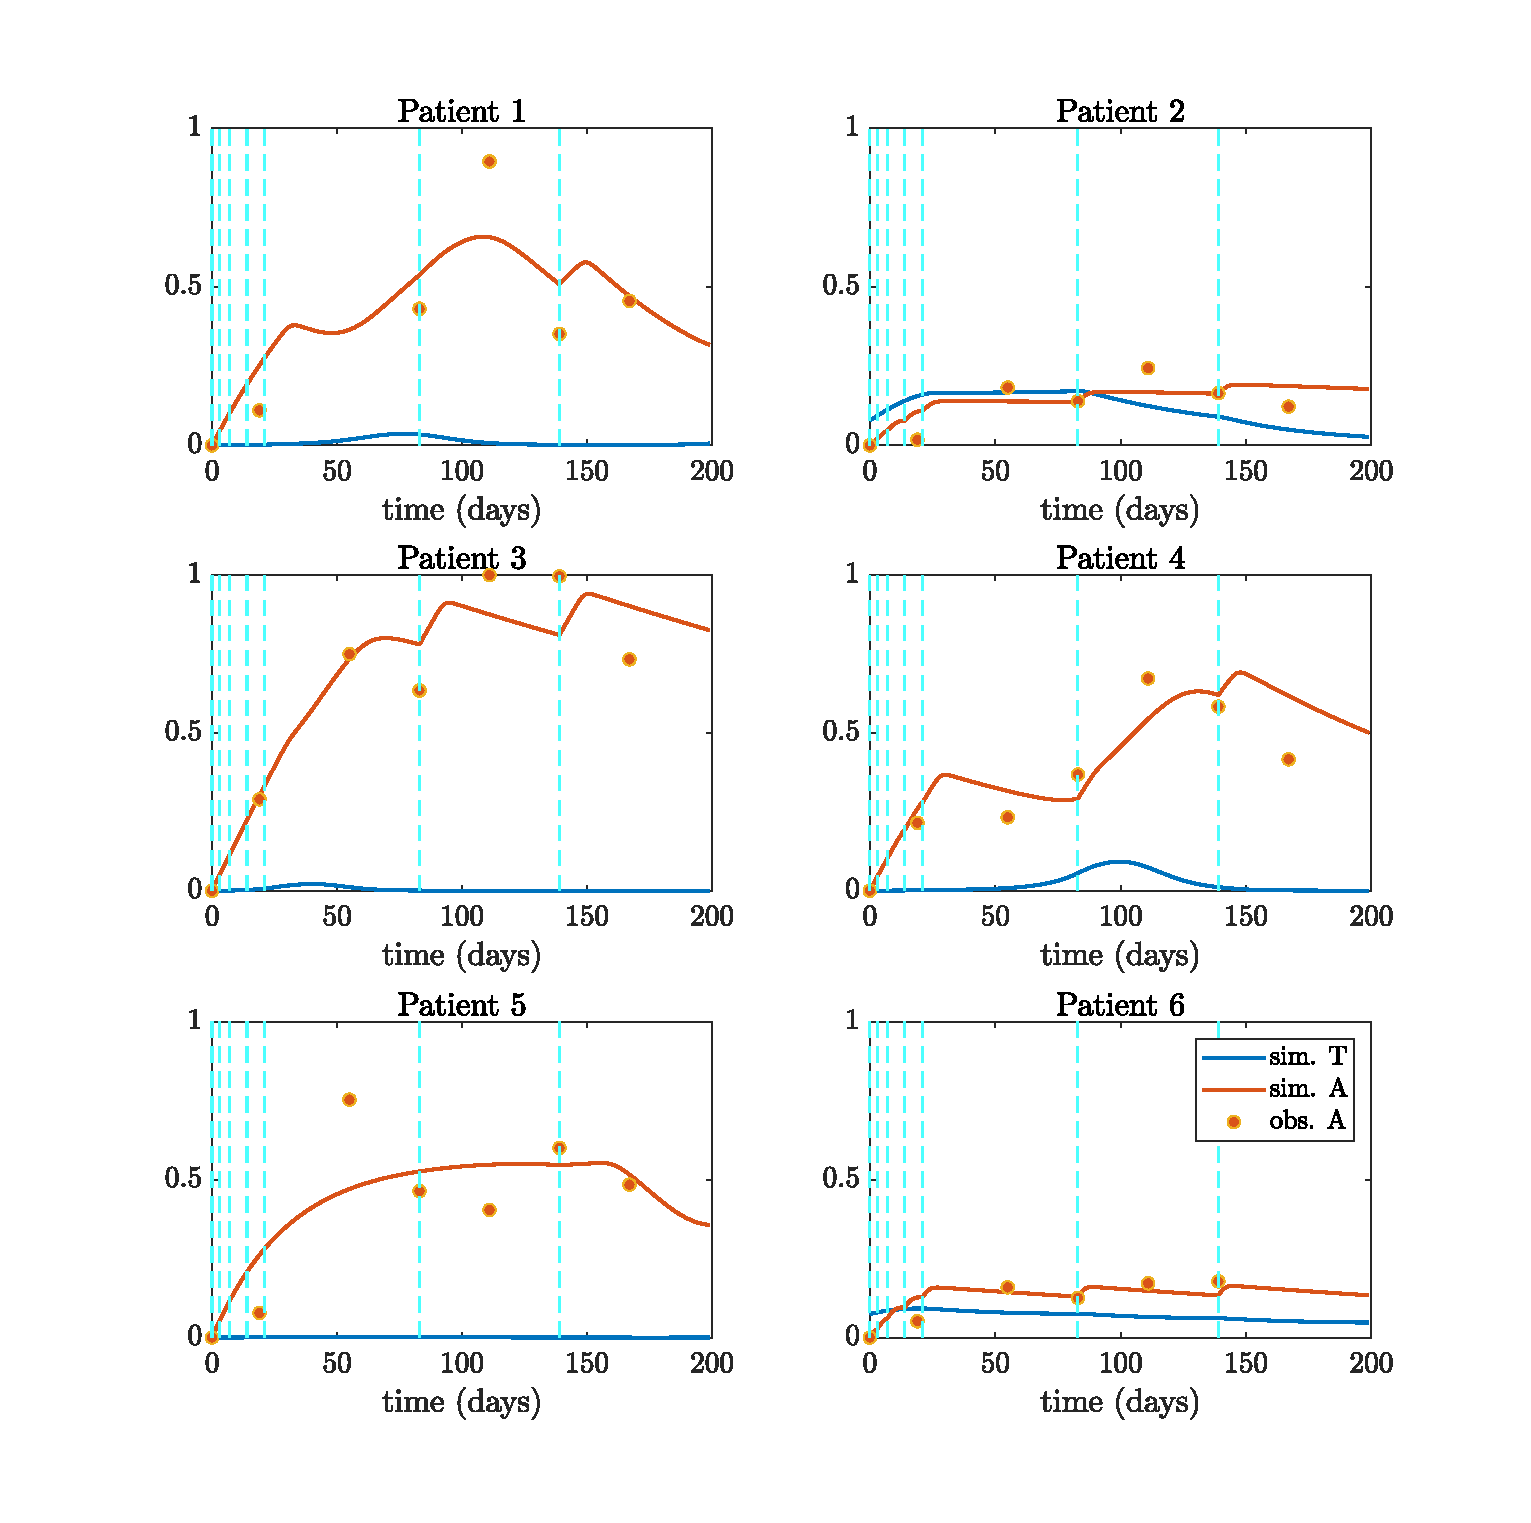
\includegraphics[width=0.7\paperwidth]{figs/pat1-6fitting}}\caption{Time course of model-simulated tumor population (sim. T) and activated T cell (sim. A) population and observed activated T cell (obs. A). Vertical bars indicate the time of cancer vaccine peptides. Tumor population and activated T cell population are scaled with tumor capacity reported by \citet{Messan2021} and the maximum observed T cell count respectively.  \label{fig:data-fitting.}}

\end{figure}

%\begin{figure}
%\centerline{\includegraphics[width=0.7\paperwidth]{\string"figs/T and A vs t\string".jpg}}
%
%\centerline{\includegraphics[width=0.7\paperwidth]{\string"figs/T and A vs t longer\string".jpg}}
%
%\caption{T and A vs time in short time (top) and longer time horizon (bottom)\label{fig:T-and-A-vs-time}}
%
%\end{figure}


\begin{table}[!t]
\centerline{
    \begin{tabular}{|c|l|l|l|l|l|l|}
    \hline
        ~ & Patient 1 & Patient 2 & Patient 3 & Patient 4 & Patient 5 & Patient 6 \\ \hline
        $\beta$  & 2.1521e-01 & 6.2241e-02 & 3.0000e-01 & 1.9441e-01 & 2.0484e-01 & 2.6810e-02 \\ \hline
        $\delta$ & 1.3507e-02 & 1.6495e-03 & 2.7590e-03 & 6.5346e-03 & 3.2821e-02 & 3.8411e-03 \\ \hline
        $s$      & 1.1362e-02 & 3.0248e-01 & 1.2712e-02 & 4.9532e-02 & 7.0630e-05 & 5.4276e-01 \\ \hline
        $\phi$   & 1.5106e-02 & 8.0486e-03 & 1.6324e-02 & 1.5038e-02 & 1.8503e-02 & 1.3204e-02  \\ \hline \hline
        RSS      & 1.1320e-01 & 1.9719e-02 & 1.0038e-01 & 7.2962e-02 & 1.4243e-01 & 8.4673e-03 \\ \hline
      RSS by MRM & 4.8800e-02 & 3.4333e-02 & 3.3667e-02 & 1.6000e-02 & 8.7000e-02 & 4.0800e-02 \\ \hline
    \end{tabular}}
\caption{\label{tab:parameters} Patient specific parameters estimated by minimizing residual sum of squares (RSS). The last row is RSS from the model by \cite{Messan2021}. Other parameters are fixed: $\delta_P=0.5,\phi=0.015,m=0.1,\lambda=2$. }
\end{table}

\section{Analysis on two types of killing terms\label{sec:Analysis-on-two}}
\subsection{Model reduction}
The dynamics of peptides $P$ is at the molecular level and
is deemed to be much faster than the cellular dynamics of $A$ and $T$.
This is also supported by parameter estimation by fitting to real
patient data (Table \ref{tab:parameters}). Thus we make quasi-steady state (QSS)
approximation for $P$ and conduct analysis in the next sections on
the reduced system below
\begin{subequations} \label{eq:2sp}
\begin{eqnarray}
A' & = & a(P)-\delta A \label{eq:A'-1}\\
T' & = & \beta T-mD(A,T)T \label{eq:T'-1}
\end{eqnarray}
\end{subequations}
where we make $P=D(A,T)T$ in (\ref{eq:A'-1}). 

To further simplifying analysis, we make another approximation that $a=\phi H(P-s)$
where $H(\cdot)$ is the Heavside step function ($H(x)=0$ if $x<0$
and $H(x)=1$ if $x\ge0$) (elaborate?). It is a limit of the Hill
function (\ref{eq:hill-a(P)}) as $\lambda\to\infty$ and facilitates the analysis conducted
in the next two sections. Approximating the Hill function by the Heaveside
step function enables us to obtain analytical results that arise from
the key anti-tumor mechanisms by T cells. This approximation
is frequently used in analyzing models of gene regulatory network
 \citep[e.g.][]{Glass1973,Mestl1995}. In \citet{Polynikis2009},
cautions have been called in using this approximation. In modeling
tumor growth, it has been used to model activation of tumor angiogenesis
factor production as a function of tumor vasculature \citep{Stamper2007},
where the authors argued that the qualitative behavior was unchanged
by this approximation. (To do: transition; details)

With QSS approximation, we have a 2-dimensional system (\ref{eq:2sp}) that is suitable
for phase plane analysis. On the phase plane, we let horizontal axis
represent $T$ and vertical axis represent $A$. We call the the curve
$D(A,T)T=s$ immune activation (IA) curve, below which $A'<0$ (population
of the activated T cells is decreasing) and above which $A'>0$ (population
of the activated T cells is growing, i.e. the immune system is activated).
Similarly, it is insightful to note that the curve $mD(A,T)T=\beta$
separates the regions of  growing or decreasing of tumor cell population. We name
$mD(A,T)T=\beta$ tumor receding (TR) curve. These two curves separate
the phase plane into four regions: 
\begin{linenomath*}
\begin{align*} 
\text{\rom{1}} &=  \{(T,A): D(A,T)T<s, D(A,T)>\beta \}; \\ 
\text{\rom{2}} &=  \{(T,A): D(A,T)T<s, D(A,T)<\beta \}; \\ 
\text{\rom{3}} &=  \{(T,A): D(A,T)T>s, D(A,T)<\beta \}; \\ 
\text{\rom{4}} &=  \{(T,A): D(A,T)T>s, D(A,T)>\beta \}. 
\end{align*}
\end{linenomath*}
The general directions of the slope field are summarized in Table \ref{tab:Four-regions}. 

On the curve $D(A,T)T=s$, the right hand side (RHS) of (\ref{eq:A'-1})
is not continuous, which may cause some issues since many classical
ODE theories are based on smoothness of the RHS. Solutions of ODE
with discontinuous RHS can be studied in a rigorous framework proposed
by \citet{Filippov1988}. Filippov's theory is mostly useful
in making sense of the solution when trajectories collide onto the
discontinuity line. However, this does not happen for our model with
either choice of the killing terms (this can be seen geometrically by looking
at the general direction of the slope field with respect to the IA
curve or algebraically verified by taking dot product of the normal
vector and the slope vector). Similar dilemma also arises when the
initial condition is on the IA curve where the slope fields on the
two sides diverge. Even though it can be resolved as a sliding solution
in the Filippov sense, this additional technicality does not offer more
biological insights. For our
purpose, we simply do not consider any initial conditions on the part of the IA
curve where this can be an issue. Furthermore, if a trajectory later reaches the IA curve, we
can assume that it crosses the curve immediately and the solution
is concatenated from one side and continued on according the RHS on
the other side. In each side of the IA curve, the system has smooth RHS and
can be analyzed using classical methods as long as the trajectory
stays on one side. (elaborate?)

\begin{table}
\centerline{%
\begin{tabular}{|c|c|c|}
\hline 
 & Tumor receding  & Tumor growing\tabularnewline
\hline 
\hline 
T cell decaying & \rom{1} \quad 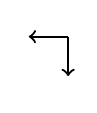
\begin{tikzpicture}[baseline=-5]
\draw[thick,->] (0,0) -- (0,-0.5);
\draw[thick,->] (0,0) -- (-0.5,0);
\addvmargin{1mm}
\end{tikzpicture} & \rom{4} \quad 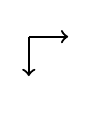
\begin{tikzpicture}[baseline=-5]
\draw[thick,->] (0,0) -- (0,-0.5);
\draw[thick,->] (0,0) -- (0.5,0);
\addvmargin{1mm}
\end{tikzpicture} \tabularnewline
\hline 
T cell growing & \rom{2} \quad 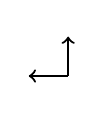
\begin{tikzpicture}[baseline=0]
\draw[thick,->] (0,0) -- (0,0.5);
\draw[thick,->] (0,0) -- (-0.5,0);
\addvmargin{1mm}
\end{tikzpicture} & \rom{3} \quad 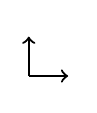
\begin{tikzpicture}[baseline=0]
\draw[thick,->] (0,0) -- (0,0.5);
\draw[thick,->] (0,0) -- (0.5,0);
\addvmargin{1mm}
\end{tikzpicture}\tabularnewline
\hline 
\end{tabular}}

\caption{\label{tab:Four-regions}Four regions on the phase plane characterized
by growing or decaying of tumor and activated T cell population. Note that since we only consider the invariant set $\Omega$
Region \rom{4} is defined to be bounded above by $\phi/\delta$.}
\end{table}


\subsection{Analysis on the law of mass action functional form}

In this case, $D(A,T)=T$ and the IA curve is $AT=s$. Above the IA
curve ($AT>s$),
\begin{eqnarray*}
A' & = & \phi-dA\\
T' & = & \beta T-mAT,
\end{eqnarray*}
and below the IA curve ($AT<s$)
\begin{subequations}
\begin{eqnarray}
A' & = & -\delta A\\
T' & = & \beta T-mAT.
\end{eqnarray}
\label{eq:belowAC}
\end{subequations}

Note that $\Omega=\{(T,A):T>0,0<A<\phi/\delta\}$ is invariant and biologically
meaningful. We focus the following analysis on $\Omega$. It is easy to deduce that
for $\frac{m\phi}{\delta}<\beta$, $A\to\frac{\phi}{\delta},T\to\infty$,
which means tumor is growing whether the immune system is activated
or off. The more interesting scenario is when $\beta<\frac{m\phi}{\delta}$,
that is, the growth rate of tumor is less than the maximum killing
rate achieved when the activate T cells reach its biologically maximum
level. This will be underlying assumption in the following analysis on law of mass action killing. 

Assuming $\beta<\frac{m\phi}{\delta}$, a trajectory starting in Region \rom{3}
enters Region \rom{4}, then enters Region \rom{1}, then enters Region \rom{2} as seen in Fig. \ref{fig:DA-PP-4regions}.
The question is whether the trajectory will enter Region \rom{3} (if it does,
there is likely a periodic solution) or stays in \rom{2}, in which case uncontrolled tumor growth is inevitable. We can derive a necessary and sufficient condition for these two cases
as follows.

In Region \rom{2}, the system evolves according to (\ref{eq:belowAC}), which
can be solved with initial condition $(T_{0},A_{0})\in\text{\rom{2}}$
exactly leading to 
\begin{eqnarray}
A(t) & = & A_{0}e^{-\delta t}\nonumber \\
T(t) & = & T_{0}\exp(\beta t-\frac{mA_{0}(1-e^{-\delta t})}{\delta})\label{eq:soln belowAC}.
\end{eqnarray}
Thus,
\begin{equation}
AT=A_{0}T_{0}\exp((\beta-\delta)t-\frac{mA_{0}}{\delta}(1-e^{-\delta t})).
\end{equation} 
If $\beta<\delta$, $AT<A_{0}T_{0}<s$ for all $t>0$ and furthermore
we have uncontrolled tumor growth $T\to\infty,A\to0$ as $t\to\infty$. This phenomenon that a small manage to grow to a large size under the radar of immune surveillance is sometimes colloquially called `sneaking through' \citep{KUZNETSOV1994}.  \cite{George2018} reported sneaking through of a slow growing tumor, which could be explained by the mechanism included in our
model. A trajectory representing a tumor sneaking through on the phase
plane is shown in the right panel of Fig. \ref{fig:PP-DA}. 

If $\beta>\delta$, the trajectory starting in Region \rom{2} reaches the IA curve 
and enters Region \rom{3}. \iffalse (to do: exists (invisible) tangential point $A_{2}^{*}=(\beta-\delta)/m$
for any $A_{0}T_{0}=s$ and $A_{0}<A^{*}$ immediately enters Region \rom{3};
). \fi So it is possible there is a periodic solution (limit cycle). Consider
the Poincare section $\{(T,A):AT=s,\beta/m<A<\phi/\delta \}$, i.e., the part of the IA curve enclosed by 
the intersection with tumor receding curve $A=\beta/m$ \iffalse (to do: or
more precisely need to consider the tangential point $A_{4}^{*}$) \fi
and the line $A=\phi / \delta$ (equilibrium of active T cells).
Since any trajectory starting from this section traverses through Regions \rom{1},\rom{2},\rom{3} and \rom{4} and must
return to this section. Hence by the fixed point theorem, there is
a fixed point, which shows the existence of a periodic solution.

For this simple case, we can further show that this fixed point is
unique. Suppose there is a periodic solution. Without loss of generality,
we assume at time $t=0$, the solution is at $(A_{0},T_{0})$ on the
IA curve where $A_{0}\in(\beta/m,\phi/\delta)$ and $A_{0}T_{0}=s$.
This periodic solution later intersects with the IA curve at $(A_{1},T_{1})$
at time $t=t_{1}$ and $(A_{2},T_{2})$ at time $t=t_{2}$. We require
$A_{2}=A_{0},T_{2}=T_{0}$ since it is periodic. We already solved
the equation below the IA curve (\ref{eq:soln belowAC}). From $A_{1}T_{1}=A_{0}T_{0}$, we
have an implicit equation for $t_{1}$ and $A_{0}$
\begin{linenomath*}
\begin{equation}
(\beta-\delta)t_{1}=\frac{mA_{0}}{\delta}(1-e^{-\delta t_{1}})\label{eq:A1T1=00003DA0T0}
\end{equation}
\end{linenomath*}
which can be shown to have a unique positive solution $t_{1}$ given $A_{0}\in(\beta/m,\phi/\delta)$ by inspecting the slope and monotonicity of both sides of the equation. 

Above the activation curve we have the solution 
\begin{linenomath*}
\begin{eqnarray*}
A & = & \frac{\phi}{\delta}-(\frac{\phi}{\delta}-A_{1})e^{-\delta t}\\
T & = & T_{1}\exp((\beta-\frac{m\phi}{\delta})t+\frac{m}{\delta}(\frac{\phi}{\delta}-A_{1})(1-e^{-\delta t})).
\end{eqnarray*}
\end{linenomath*}
From $A_{2}=A_{0}$, we have 
\begin{linenomath*}
\begin{equation}
e^{\delta t_{2}}(\frac{\phi}{\delta}-A_{0})=\frac{\phi}{\delta}-A_{0}e^{-\delta t_{1}}.\label{eq:A2=00003DA0}
\end{equation}
\end{linenomath*}
From $T_{2}=T_{0}$, we have
\begin{linenomath*} 
\begin{equation}
(\beta-\frac{m\phi}{\delta})t_{2}+\frac{m}{\delta}(\frac{\phi}{\delta}-A_{1})(1-e^{-\delta t_{2}})+\beta t_{1}-\frac{m}{\delta}A_{0}(1-e^{-\delta t_{1}})=0\label{eq:T2=00003DT0}
\end{equation}
\end{linenomath*}
where $A_{1}=A_{0}e^{-\delta t_{1}}$. We have three nonlinear equations (\ref{eq:A1T1=00003DA0T0}),
(\ref{eq:A2=00003DA0}) and (\ref{eq:T2=00003DT0}) for three unkowns
$t_{1},t_{2}$ and $A_{0}$. In general there is no guarantee of existence
of an unique solution. For this specific case, however, we can first
eliminate the exponentials $e^{-\delta t_{1}}$ and $e^{-\delta t_{2}}$,
which gives 
\begin{linenomath*}
\[
\frac{t_{2}}{t_{1}}=\frac{\beta\delta}{m\phi-\beta\delta}.
\]
\end{linenomath*}
Let $\gamma=\frac{\beta\delta}{m\phi-\beta\delta}$. Note that $\gamma>0$
from the previous assumptions. So we can eliminate $A_{0}$ and $t_{2}$
and reach an equation for $t_{1}$
\begin{linenomath*}
\begin{equation}
\frac{(e^{\gamma t_{1}}-1)(1-e^{-t_{1}})}{e^{\gamma t_{1}}-e^{-t_{1}}}=\frac{\beta-\delta}{m\phi/\delta^{2}}t_{1}\label{eq:t1-period}
\end{equation}
\end{linenomath*}
which can be shown to have an unique solution. Let 
\begin{linenomath*}
\begin{equation}
f(t_{1})=\frac{(e^{\gamma t_{1}}-1)(1-e^{-t_{1}})}{e^{\gamma t_{1}}-e^{-t_{1}}}.\label{eq:f(t1)}
\end{equation}
\end{linenomath*}
It can be shown that $f'(t)>0$ and $f''(t)<0$ for all $t>0$ (see
details of calculation in the appendix), and $\lim_{t\to0}f'(t)=\frac{\beta}{m\phi/\delta^{2}}>\frac{\beta-\delta}{m\phi/\delta^{2}}$.
Moreover, $\lim_{t\to\infty}f(t)=1$. It follows that the periodic
solution is unique. Moreover, (\ref{eq:t1-period}) can be readily
solved numerically to give the length of a period given parameters
as shown in Figure (\ref{fig:Contour-plot-of-period}). It is interesting
to notice that the period is independent from the threshold $s$.
It may just be a mathematical consequence and not bear any biological
meaning. 




\begin{figure}
\centerline{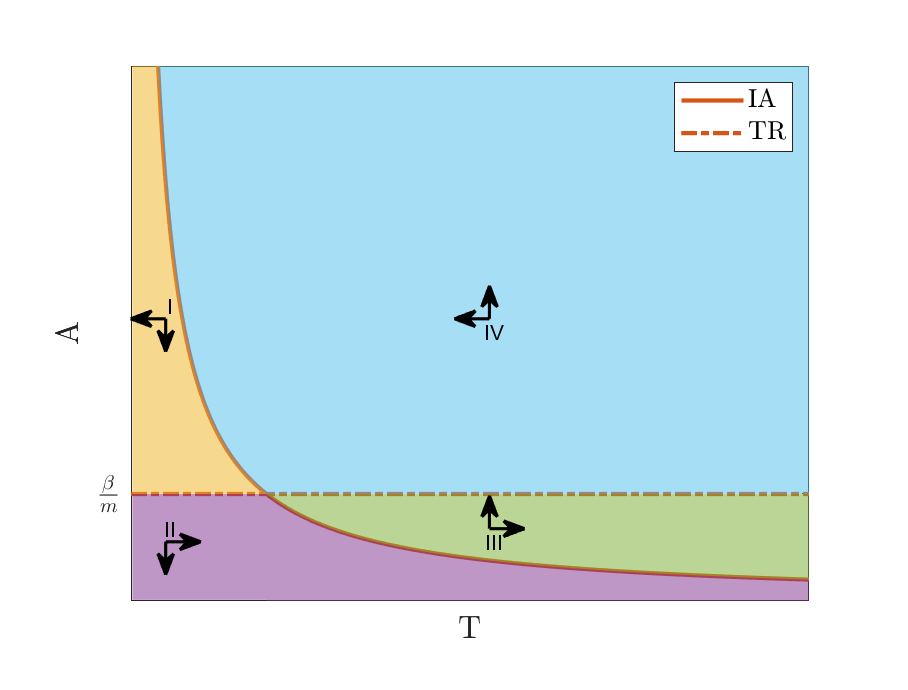
\includegraphics[width=1\linewidth]{figs/DA-colored-regions}}

\caption{Four regions (\rom{1}, \rom{2}, \rom{3} and \rom{4}) on the phase plane of (\ref{eq:2sp}) with the law of mass action killing $D(A,T)=A$. The phase plane is divided by immune activation (IA) curve and tumor receding curve (TR) into four regions, which are 
shaded in different colors. General directions of the slope field
are indicated by arrows.  \label{fig:DA-PP-4regions}}
\end{figure}

\begin{figure}
\centerline{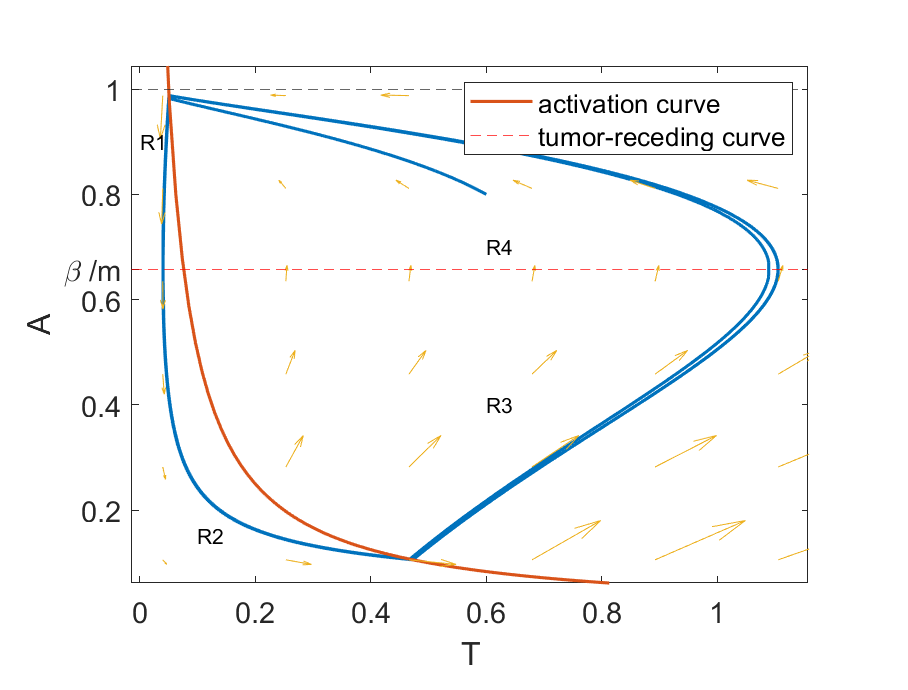
\includegraphics[width=0.3\paperwidth]{figs/phase_plane_periodic_DA}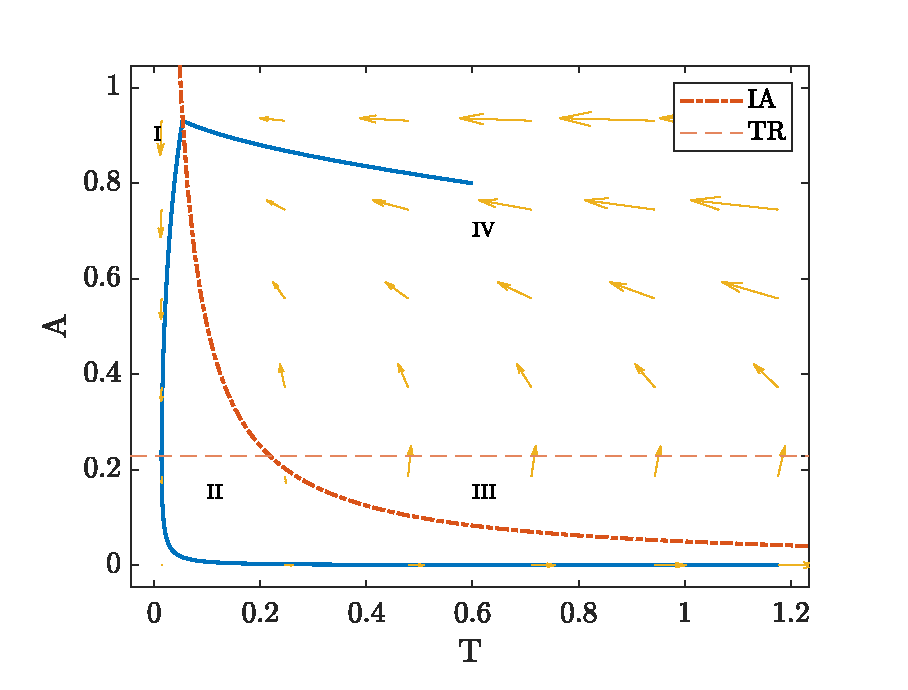
\includegraphics[width=0.3\paperwidth]{figs/phase_plane_sneakthru_DA}}
\caption{A exemplary trajectory (solid line) on the phase plane of (\ref{eq:2sp}) with the law of mass action killing $D(A,T)=A$. Left: a periodic solution exists if $\beta>\delta$;
right:tumor sneak-through when $\beta<\delta$.\label{fig:PP-DA} }
\end{figure}

\begin{figure}
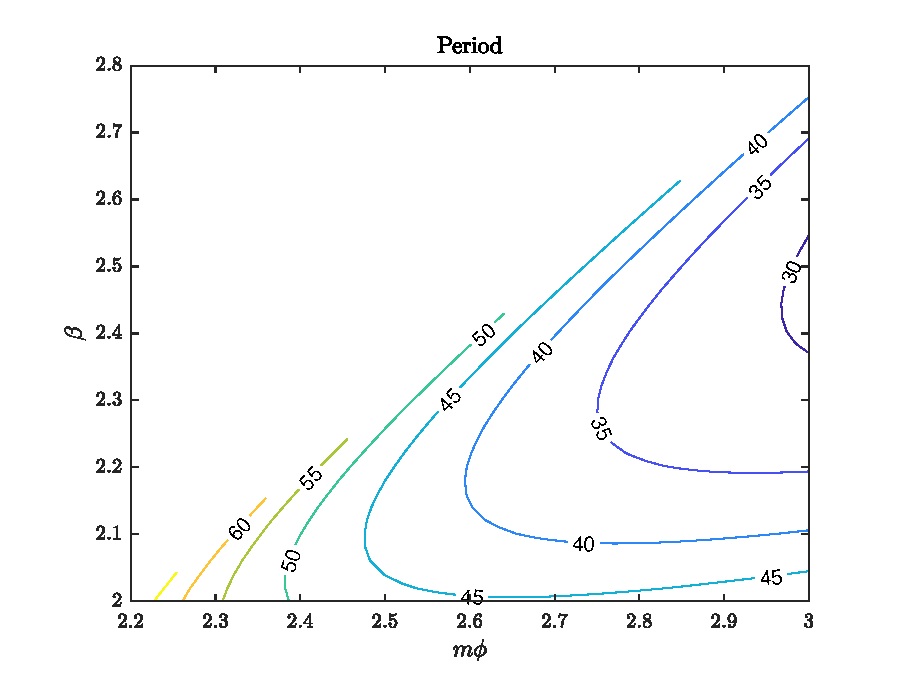
\includegraphics[width=0.9\linewidth]{figs/DA-period-contour}
\caption{\label{fig:Contour-plot-of-period}Contour plot of period computed
from (\ref{eq:t1-period}). The period is dimensionless with time scale
with $1/delta$. Same scale is applied to the parameter $\beta,m,\phi$. }
\end{figure}


\subsection{Analysis on the dePillis-Radunskaya Law functional form}

In this section, we analyze the system (\ref{eq:T'-1}) with $D$
defined as (\ref{eq:PR law-1}). Note that $D$ is in fact a Hill
function of ratio $A/T$, in which $n$ describes how fast per capita
killing rate turns on as the ratio of activated T cells verse tumor cells increase.
The implications of $n$ on uncontrolled tumor growth will be derived later in this section.
First, we look at the IA curve and the TR curve and define the four
regions (Table \ref{tab:Four-regions}) similar to what we did in
the previous section. As in the previous section, we focus on the
invariant set $\{(T,A):T>0,0<A<\phi/d\}$. We assume $\beta<m$, i.e.,
the growth rate of tumor is smaller than the maximum killing rate.
Otherwise the tumor grows exponentially regardless of immune control.
Even though we still have simple analytical solution of $A$, analytical
solutions of $T$ are not tractable. We seek a sufficient condition
of uncontrolled tumor growth if the initial condition is in Region \rom{2}. 

The IA curve for dePillis-Radunskaya Law is
\begin{eqnarray}
\frac{1}{s}A^{n}T & = & k^{n}T^{n}+A^{n}\label{eq:IA-dP}
\end{eqnarray}
which has an asymptote $T=1/s$. Consider here $n>1$. \iffalse (to do: $n=1$?) \fi
By implicit differentiation of (\ref{eq:IA-dP}), it can be found
that the IA curve achieves a minimum at $T=\frac{n}{n-1}s$, at which
$A=ks(n-1)^{1/n}\frac{n}{n-1}$. Note that $T'=(\beta-mD(A,T))T>0$
if $\beta>mD(A,T)$ and vice versa, i.e., above the TR curve the tumor
is receding and above it the tumor is receding. Moreover, the TR curve
$\beta=mD(A,T)$ is now a line pass the origin with slope 
\begin{linenomath*}
\[
\frac{k}{(m/\beta-1)^{1/n}}
\]
\end{linenomath*}
There is a unique intersection ($T=\frac{sm}{\beta}$) between the
TR line and the IA curve in the invariant set $\Omega$ if 
\begin{eqnarray}
s & < & \frac{\beta}{m}\frac{\phi}{k\delta}(\frac{m}{\beta}-1)^{1/n}\label{eq:s<}
\end{eqnarray}
  Otherwise, Region \rom{3} does not exist and the tumor population $T$ grows
without bound for any initial condition in Region \rom{2}. 

Suppose the interaction of the IA and TR curves exists in $\Omega$. We can derive
a sufficient condition for uncontrolled tumor growth. If the intersection
is on the right to the minimum of the IA curve, then the minimum is above the line
and hence any trajectory starting in Region \rom{2} cannot cross the IA curve
since $A$ is monotonically decreasing. Thus the sufficient condition
of uncontrolled tumor growth is 
\begin{linenomath*}
\begin{equation}
\frac{m}{\beta}>\frac{n}{n-1}.\label{eq:sneak-thru-cond}
\end{equation}
\end{linenomath*}
Since we have assumed $m>\beta$, this condition is satisfied for sufficient large $n$. In this sense, a faster switch in the dePillis-Radunskaya
Law favors uncontrolled tumor growth. Since $n$ also controls the tail of the Hill function, a better  interpretation may be that
not enough killing at the low $A/T$ tail favors uncontrolled tumor growth. 

Now consider a trajectory started in Region \rom{1} with $A(0)>\frac{n}{n-1}s$ (this extra constraint on the initial condition precludes the "pathological" case in which the trajectory goes to Region \rom{4}),
Note that in Region \rom{1} both $A'<0$ and $T'<0$. We want to study whether we have $T\to0$ and its condition if it does. Since (\ref{eq:PR law-1}) is not defined at $A=T=0$, we consider
a transformation $x=A/T$, which gives  
\begin{linenomath*}
\begin{eqnarray}
x' & = & x(-\delta-\beta+\frac{mx^{n}}{k^{n}+x^{n}})\label{eq:x' for dP}\\
 & = & \frac{x}{k^{n}+x^{n}}((m-\delta-\beta)x^{n}-(\delta+\beta)k^{n})\nonumber 
\end{eqnarray}
\end{linenomath*}
Note that for $m\le\delta+\beta$, $x'<0$ and there exists $\tau$
such that $x(\tau)=\frac{k}{(m/\beta-1)^{1/n}}$ for any $x(0)>\frac{k}{(m/\beta-1)^{1/n}}$.
Thus, the trajectory must enter Region \rom{2}. For $m>\delta+\beta$, it can
be shown that 
\begin{linenomath*}
\[
x_{1}^{*}=\frac{k}{(m/(\delta+\beta)-1)^{1/n}}
\]
\end{linenomath*}
 is a unstable fixed point of (\ref{eq:x' for dP}). Also note that
$x_{1}^{*}>\frac{k}{(m/\beta-1)^{1/n}}$ , the slope of $\beta=mD(A,T)$.
If $x(0)<x_{1}^{*}$, $x\to0$, in which case the trajectory enters
R2. If $x(0)>x_{1}^{*},x\to\infty$, in which case the trajectory
will not cross the line $\beta=mD(A,T)$ to enter Region \rom{2} and $T\to0$
faster than $A$ does. This is the case that the tumor is eliminated.
The line $A=x_{1}^{*}T$ is the separtrix that separates these two cases
as depicted in Figure \ref{fig:dP-PP-sep}. In contrast with the law
of mass action killing, the tumor can be completely eliminated under the
dePillis-Radunskaya Law as long as the maximum killing is large enough
and the starting point is favorable, i.e. the tumor is not too large
compared to the active T cell population. 

Now we consider trajectories starting in Region \rom{3}.  \iffalse (can show no pseudo-equilibrium;
tangent points are invisible? see Appendix) \fi Sufficient and necessary
conditions for characterizing the destiny of trajectory are elusive.
Instead, we seek for sufficient conditions. Let the initial condition $A(0)=A_0$ and $T(0)=T_0$.
With $x=A/T$, 
\begin{eqnarray*}
x' & = & x(\frac{\phi}{A}-\delta-\beta+\frac{mx^{n}}{k^{n}+x^{n}})\\
A' & = & \phi-\delta A.
\end{eqnarray*}
Since $A$ is monotonically increasing,
\begin{eqnarray*}
x' & \le & x(\frac{\phi}{A_{0}}-\delta-\beta+\frac{mx^{n}}{k^{n}+x^{n}})\\
   & = & \frac{x}{k^{n}+x^{n}}((m+\frac{\phi}{A_{0}}-\delta-\beta)x^{n}-(\delta+\beta-\frac{\phi}{A_{0}})k^{n}).
\end{eqnarray*}
There are two conditions can be deduced from the above inequality, either of which is sufficient for the trajectory
to enter Region \rom{2}: One is $\delta+\beta-\frac{\phi}{A_{0}}>m$; For $0<\delta+\beta-\frac{\phi}{A_{0}}<m$,
$x_{3}^{*}=k(\frac{\delta+\beta-\phi/A_{0}}{m+\phi/A_{0}-\delta-\beta})^{1/n}$ is an unstable fixed point. Thus for a trajectory starting in Region \rom{3} with $A_0/T_0<x_{3}^{*}$,
it enters Region \rom{2}. A third sufficient condition can be deduced from the phase plane (Fig. \ref{fig:dP-PP-4regions}), if $T_0>\frac{\phi}{\delta k}(\frac{m}{\beta}-1)^{1/n}$, the trajectory must enter Region \rom{2}. 

Also note that given $A_0$, $T_0$ can be chosen to make the initial point sufficiently close to the TR line so that the trajectory then crosses the line $\beta=mD(A,T)$
to enter Region \rom{4}. Moreover, once in Region \rom{4} this trajectory continues to enter Region \rom{1}. In fact, any trajectory starting in Region \rom{4} enters Region \rom{1}. 

We have gained biologically interpretable results by analyzing the system \ref{eq:2sp} with the dePillis-Radunskaya Law kill \ref{eq:PR law-1} region by region. We stop here and remark that an explicit global condition for this system is likely to be complicated if achievable.  Our findings and its biological interpretation will be discussed in the next section.

\begin{figure}
\centerline{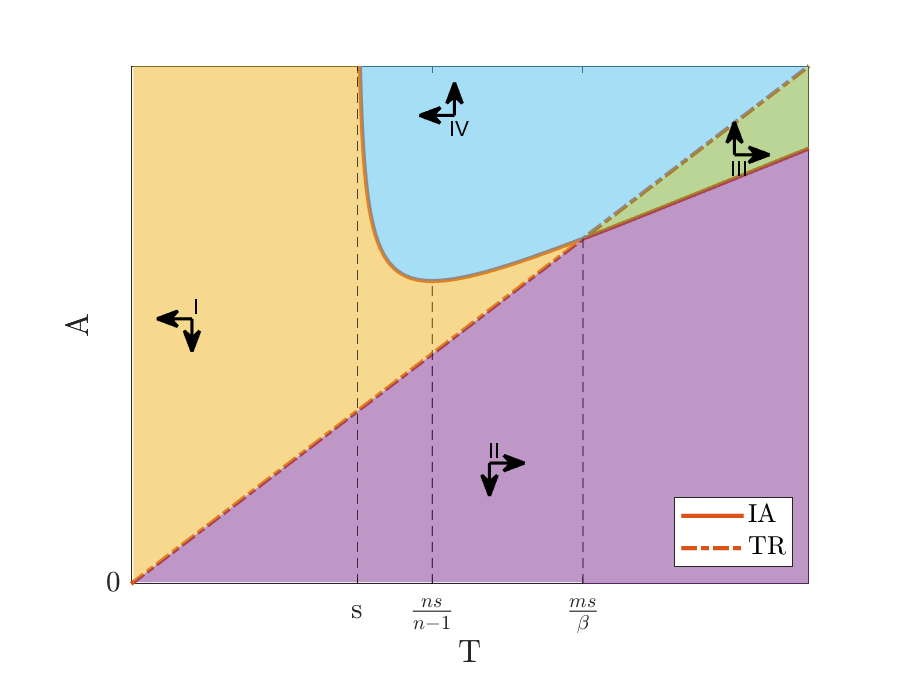
\includegraphics[width=0.5\linewidth]{figs/dP-colored-regions-l}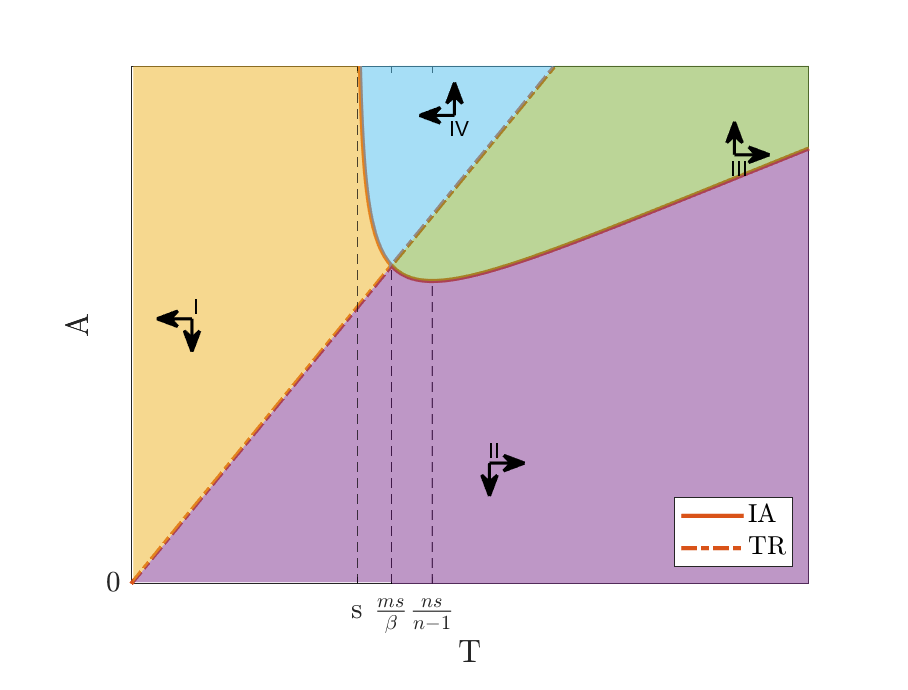
\includegraphics[width=0.5\linewidth]{figs/dP-colored-regions-r}}

\caption{\label{fig:dP-PP-4regions}
Four regions (\rom{1}, \rom{2}, \rom{3} and \rom{4}) on the phase plane of (\ref{eq:2sp}) with the the dePillis-Radunskaya Law (\ref{eq:PR law-1}). The phase plane is divided by immune activation (IA) curve and tumor receding curve (TR) into four regions, which are 
shaded in different colors. General directions of the slope field
are indicated by arrows. Left: $\frac{m}{\beta}>\frac{n}{n-1}$
is sufficient for tumor to sneak through; right: when $\frac{m}{\beta}<\frac{n}{n-1}$
, it requires further investigation whether a trajectory will enter
Region \rom{3} from Region \rom{2}. }
\end{figure}

\begin{figure}
\centerline{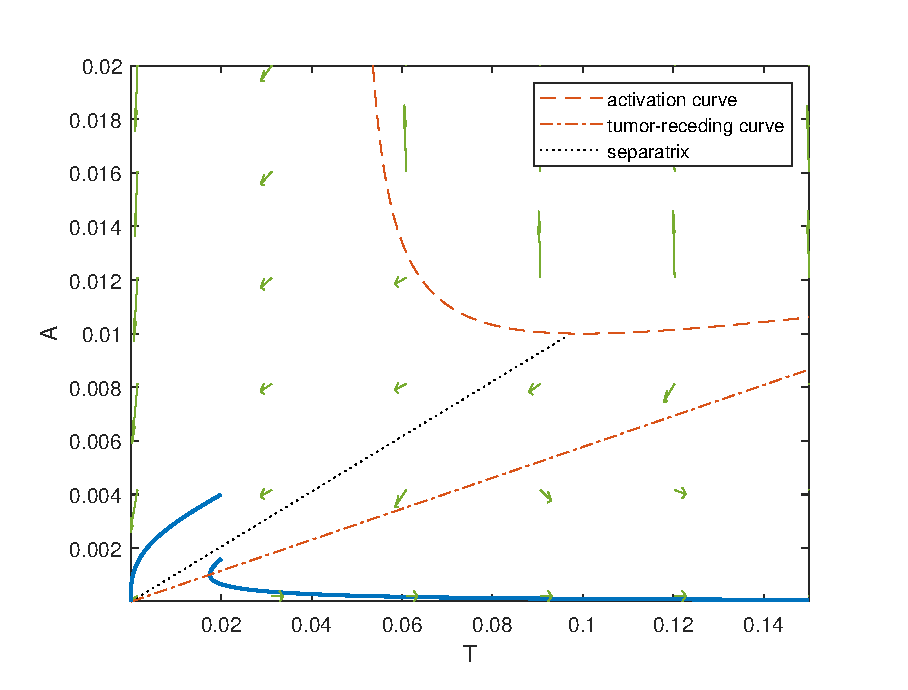
\includegraphics[width=0.7\linewidth]{figs/dP-PP-sep}}

\caption{\label{fig:dP-PP-sep}Tumor elimination of system (\ref{eq:2sp}) with the the dePillis-Radunskaya Law (\ref{eq:PR law-1}) depending on the initial condition
in Region \rom{1}. The trajectory starting above the separatrix represents tumor
elimination while the one starts below it enters Region \rom{2} and represents
uncontrolled tumor growth. }
\end{figure}


\section{Discussion\label{sec:Discussion}}

To understand tumor-immune interaction, we introduce a simple model as
an alternative to the one proposed by \citet{Messan2021}. Its simplisty allows us to investigate two common choices for the killing term analytically. By QSS argument,
we reduce the model into two equations which are amendable to phase
plane analysis. A further approximation is taken by replacing the
Hill function representing activation of T cells in presence of neoantigen
peptides. We recognize two important curves that separate the phase
plane into four regions where the system evolves distinctively. Simple
geometrical arguments based on this categorization and some basic
calculations lead to meaningful characterization of the model behavior.
The clear analytical results facilitate interpretation of the tumor
progression or elimination as a consequence of the given mechanism.
Particularly, for the law of mass action killing, we have derived
that $\beta<\delta$, i.e. the tumor growth rate is slower than the
decaying rate of active T cells, as a necessary and sufficient condition
for uncontrolled tumor growth. In a strict sense, tumor `sneaking through'
is a phenomenology that the tumor exhibits a dormant period during which the
tumor size remains small and eventually grow large escaping the immune control. It has been heavily studied theoretically
and experimentally \citep[see e.g.][for a review]{Wilkie2013}. Recently,
slow growth induced `sneaking through' is reported in \cite{George2018}.
In addition to their findings, our model offers an alternative mechanism
that could explains sneaking through of a slowing growing tumor. Our model is based on the hypothesis that the neoantigen peptides released by lyisis of the tumor cells are the signal that triggers immune response. Based on our findings, cancer neoantigen vaccines are an effective treatment for `sneaking through' tumors.   

In comparison to the law of mass action killing, the dePillis-Radunskaya
Law offers richer dynamics as well as more challenging analysis. The
dePillis-Radunskaya Law is essentially a ratio-dependent Hill function.
Ratio-dependent functional responses have been the focus of plenty
of analytical work in the context of ecology \citep{Abrams2000,Hsu2001,Hsu2003}.
In comparison, less analysis has been conducted for models of cancer
immunology. This work is a step to fill this gap. In approximating
the Hill function in activation of T cells as a hard switch, we are
able to focus on the switching speed of the Hill function employed
in the dePillis-Radunskaya Law. A salient sufficient condition (\ref{eq:sneak-thru-cond}) for
uncontrolled tumor growth is directly related to $n$ in (\ref{eq:PR law-1}), which states that large $n$ enables
uncontrolled tumor growth. It may be better to interpret this result as ``not
enough killing at low $A/T$ tail makes uncontrolled growth possible''.
In contrast to the law of mass action killing for which asymptotic
result does not depend on initial condition, under the dePillis-Radunskaya
Law, tumor elimination is possible and may depends on the initial
condition. It informs the necessity of medical intervention to get
the patient into the favorable initial condition that may lead to
a cure. This observation also supports the common medical practice
that uses cancer vaccine as an adjuvant therapy after the primary
tumor is reduced by surgery or radiotherapy.

The choice of making peptides $P$ as the QSS variable is justified
by the estimated parameter values and the belief that its dynamics on the molecular
level is faster than dynamics on the cellular level on which $A$
and $T$ operate. However, it is a key component as dosage of cancer
vaccine is modeled as a time-dependent source term in (\ref{eq:P'}).
Treating $P$ as a QSS variable makes it impossible to study dosing
explicitly in our reduced model. Nevertheless, it should be noted
that continuous dosing, i.e. constant $u(t)$, is equivalent to a
change to the threshold parameter $s$. Specifically, increasing the
constant dose is equivalent to lowering the threshold $s$ and vice
verse. In characterizing the model behavior, $s$ seemly does not
play a role in most the results we derived. But likely it is expected
to be important biologically. First, we point out that it is indeed
an important parameter in deciding if the IA and TR curve have an
intersection when the the dePillis-Radunskaya Law is used. As higher
dosage favors the inequality (\ref{eq:s<}), it assists in taking
tumor back to control (crossing the TR line from below). Furthermore,
even though $s$ does not appear in the conditions for asymptotic
results, it is an important control parameter in determining the size
of tumor in the periodic solution or a transient solution to elimination.
The existence of a periodic solution as seen in the reduced model
is also found in the full model. But numerical experiment shows its
period differs in a large amount from the reduced model. That being
said, we do recognize the undesirable limitation of the current QSS
approximation in studying dosing strategy as well as its effects on
the quantities that is of medical interests in comparison to the full
model (\ref{eq:P'}). It is left to future study to investigate and
overcome these issues. 

\section*{Appendix}

\subsection*{Proof of $f'(t)>0$ and $f''(t)>0$ }

Let $x=e^{t_{1}}$. Note that $x>1$. 
\begin{eqnarray*}
\frac{df}{dx} & = & \frac{x^{1+\gamma}(-2(1+\gamma)+\gamma x+\frac{\gamma}{x}+x^{\gamma}+\frac{1}{x^{\gamma}})}{(x^{1+\gamma}-1)^{2}}>0\\
\frac{d^{2}f}{dx^{2}} & = & \frac{x^{\gamma-2}(-2x^{2}(x^{\gamma}-1)^{2}-\gamma^{2}(x-1)^{2}(x^{1+\gamma}+1)-\gamma(x-1)(1+3x-5x^{1+\gamma}+x^{2+\gamma}))}{(x^{1+\gamma}-1)^{3}}
\end{eqnarray*}
we will focus the part of the numerator inside the parenthesis. 
\begin{align*}
 & -2x^{2}(x^{\gamma}-1)^{2}-\gamma^{2}(x-1)^{2}(x^{1+\gamma}+1)-\gamma(x-1)(1+3x-5x^{1+\gamma}+x^{2+\gamma})\\
\le & -2\sqrt{2}x(x^{\gamma}-1)\gamma(x-1)\sqrt{x^{1+\gamma}+1}-\gamma(x-1)(1+3x-5x^{1+\gamma}+x^{2+\gamma})\\
= & -\gamma(x-1)(2\sqrt{2}x(x^{\gamma}-1)\sqrt{x^{1+\gamma}+1}+1+3x-5x^{1+\gamma}+x^{2+\gamma}\\
\le & -\gamma(x-1)(1-x-x^{1+\gamma}+x^{2+\gamma})\\
< & 0
\end{align*}
where we used the fact $-a^{2}-b^{2}<-2ab$ and $x>1$. 

\subsection*{no pseudo-equilibrium for dePillis-Radunskaya Law (work in progress)}

The IA curve $D(A,T)T=s$ has its normal vector $\mathbf{n}=(\frac{\partial D}{\partial T}T+D,\frac{\partial D}{\partial A}T)$
pointing into the region $D(A,T)T>s$, where $T\frac{\partial D}{\partial A}>0$
and $\frac{\partial D}{\partial T}T+D$ changes its sign at $T=\frac{n}{n-1}s$,
i.e. $\frac{\partial D}{\partial T}T+D$\textgreater 0 for $T\in(s,\frac{n}{n-1}s)$
. Above the IA, we have slope field $\mathbf{v}^{+}=(T(\beta-mD),\phi-dA).$
Below the IA, we have the slope field $\mathbf{v}^{-}=(T(\beta-mD),-dA).$
Thus $\mathbf{v}^{+}\cdot\mathbf{n}=\mathbf{v}^{-}\cdot\mathbf{n}+\phi T\frac{\partial D}{A}$.
It follows that $|\mathbf{v}^{+}\cdot\mathbf{n}|+|\mathbf{v}^{-}\cdot\mathbf{n}|\ne0$
(cannot be zero at the same time). Moreover, if $\mathbf{v}^{+}\cdot\mathbf{n}=0$,
$\mathbf{v}^{-}\cdot\mathbf{n}<0$; if $\mathbf{v}^{-}\cdot\mathbf{n}=0$,
$\mathbf{v}^{-}\cdot\mathbf{n}>0$.

\subsection*{unique tangential point}
To do: move the part below to appendix? 

There is a unique tangential point $A_{4}^{*}$ in R4. Let $x=AT$,
we have $x'=x(\frac{\phi}{A}-mA+\beta-\delta)$. Consider the polynomial
$p(A)=-mA^{2}+(\beta-\delta)A+\phi$, which has exactly one positive
root $A_{4}^{*}$. Trajectory leaves R4 if $A>A_{4}^{*}$. Note that
$A_{4}^{*}>\beta/m$ by verifying that $p(\beta/m)>0$. There is also
a unique tangential point $A_{2}^{*}$ in R2 if $\beta>\delta$. Again
let $x=AT$. We have $x'=x(\beta-\delta-mA)$. It follows that $A_{2}^{*}=\frac{\beta-\delta}{m}$. 

\bibliography{export}

\end{document}